\section{\projectName}\label{sec:projectDesign}
The following sections will illustrate \projectName~and all of its features. We also illustrate the decisions taken to be able to create this tool. We will start by explaining the general theory behind the approach, to then move onto the general architecture, the server side components, and then the client side components. 

\subsection{Overview}

A graph is a collection of nodes, which form a network. If we consider the world wide web, we can represent each page as a node inside of that network. When a connection exists from a page to another, for example with a link, we can say that the two pages are connected and an edge between them is created. 

The same reasoning can be applied to a document. Each part of the document becomes a node, and the edges between the different nodes in the network represent the similarity between the parts of the document. To provide a relationship between the nodes and the data displayed, we introduce the notion of an information unit. An information unit is a piece of content extracted from a page, which can contain either code or plain text.

In our approach, an information unit is a paragraph where the content can either be plain text, or code. The construction of the edges is the same as \cite{Ponz2015b}, and relies on the H-AST nodes composing the information units.  

To create the extractive summary, a possible approach consists in using HoliRank to calculate the degree of centrality of each information unit in the graph, and then select the most central ones according to a threshold set by the user. An example of this process can be seen in Figure \ref{fig:graph}.

\begin{figure}[H]
\centering
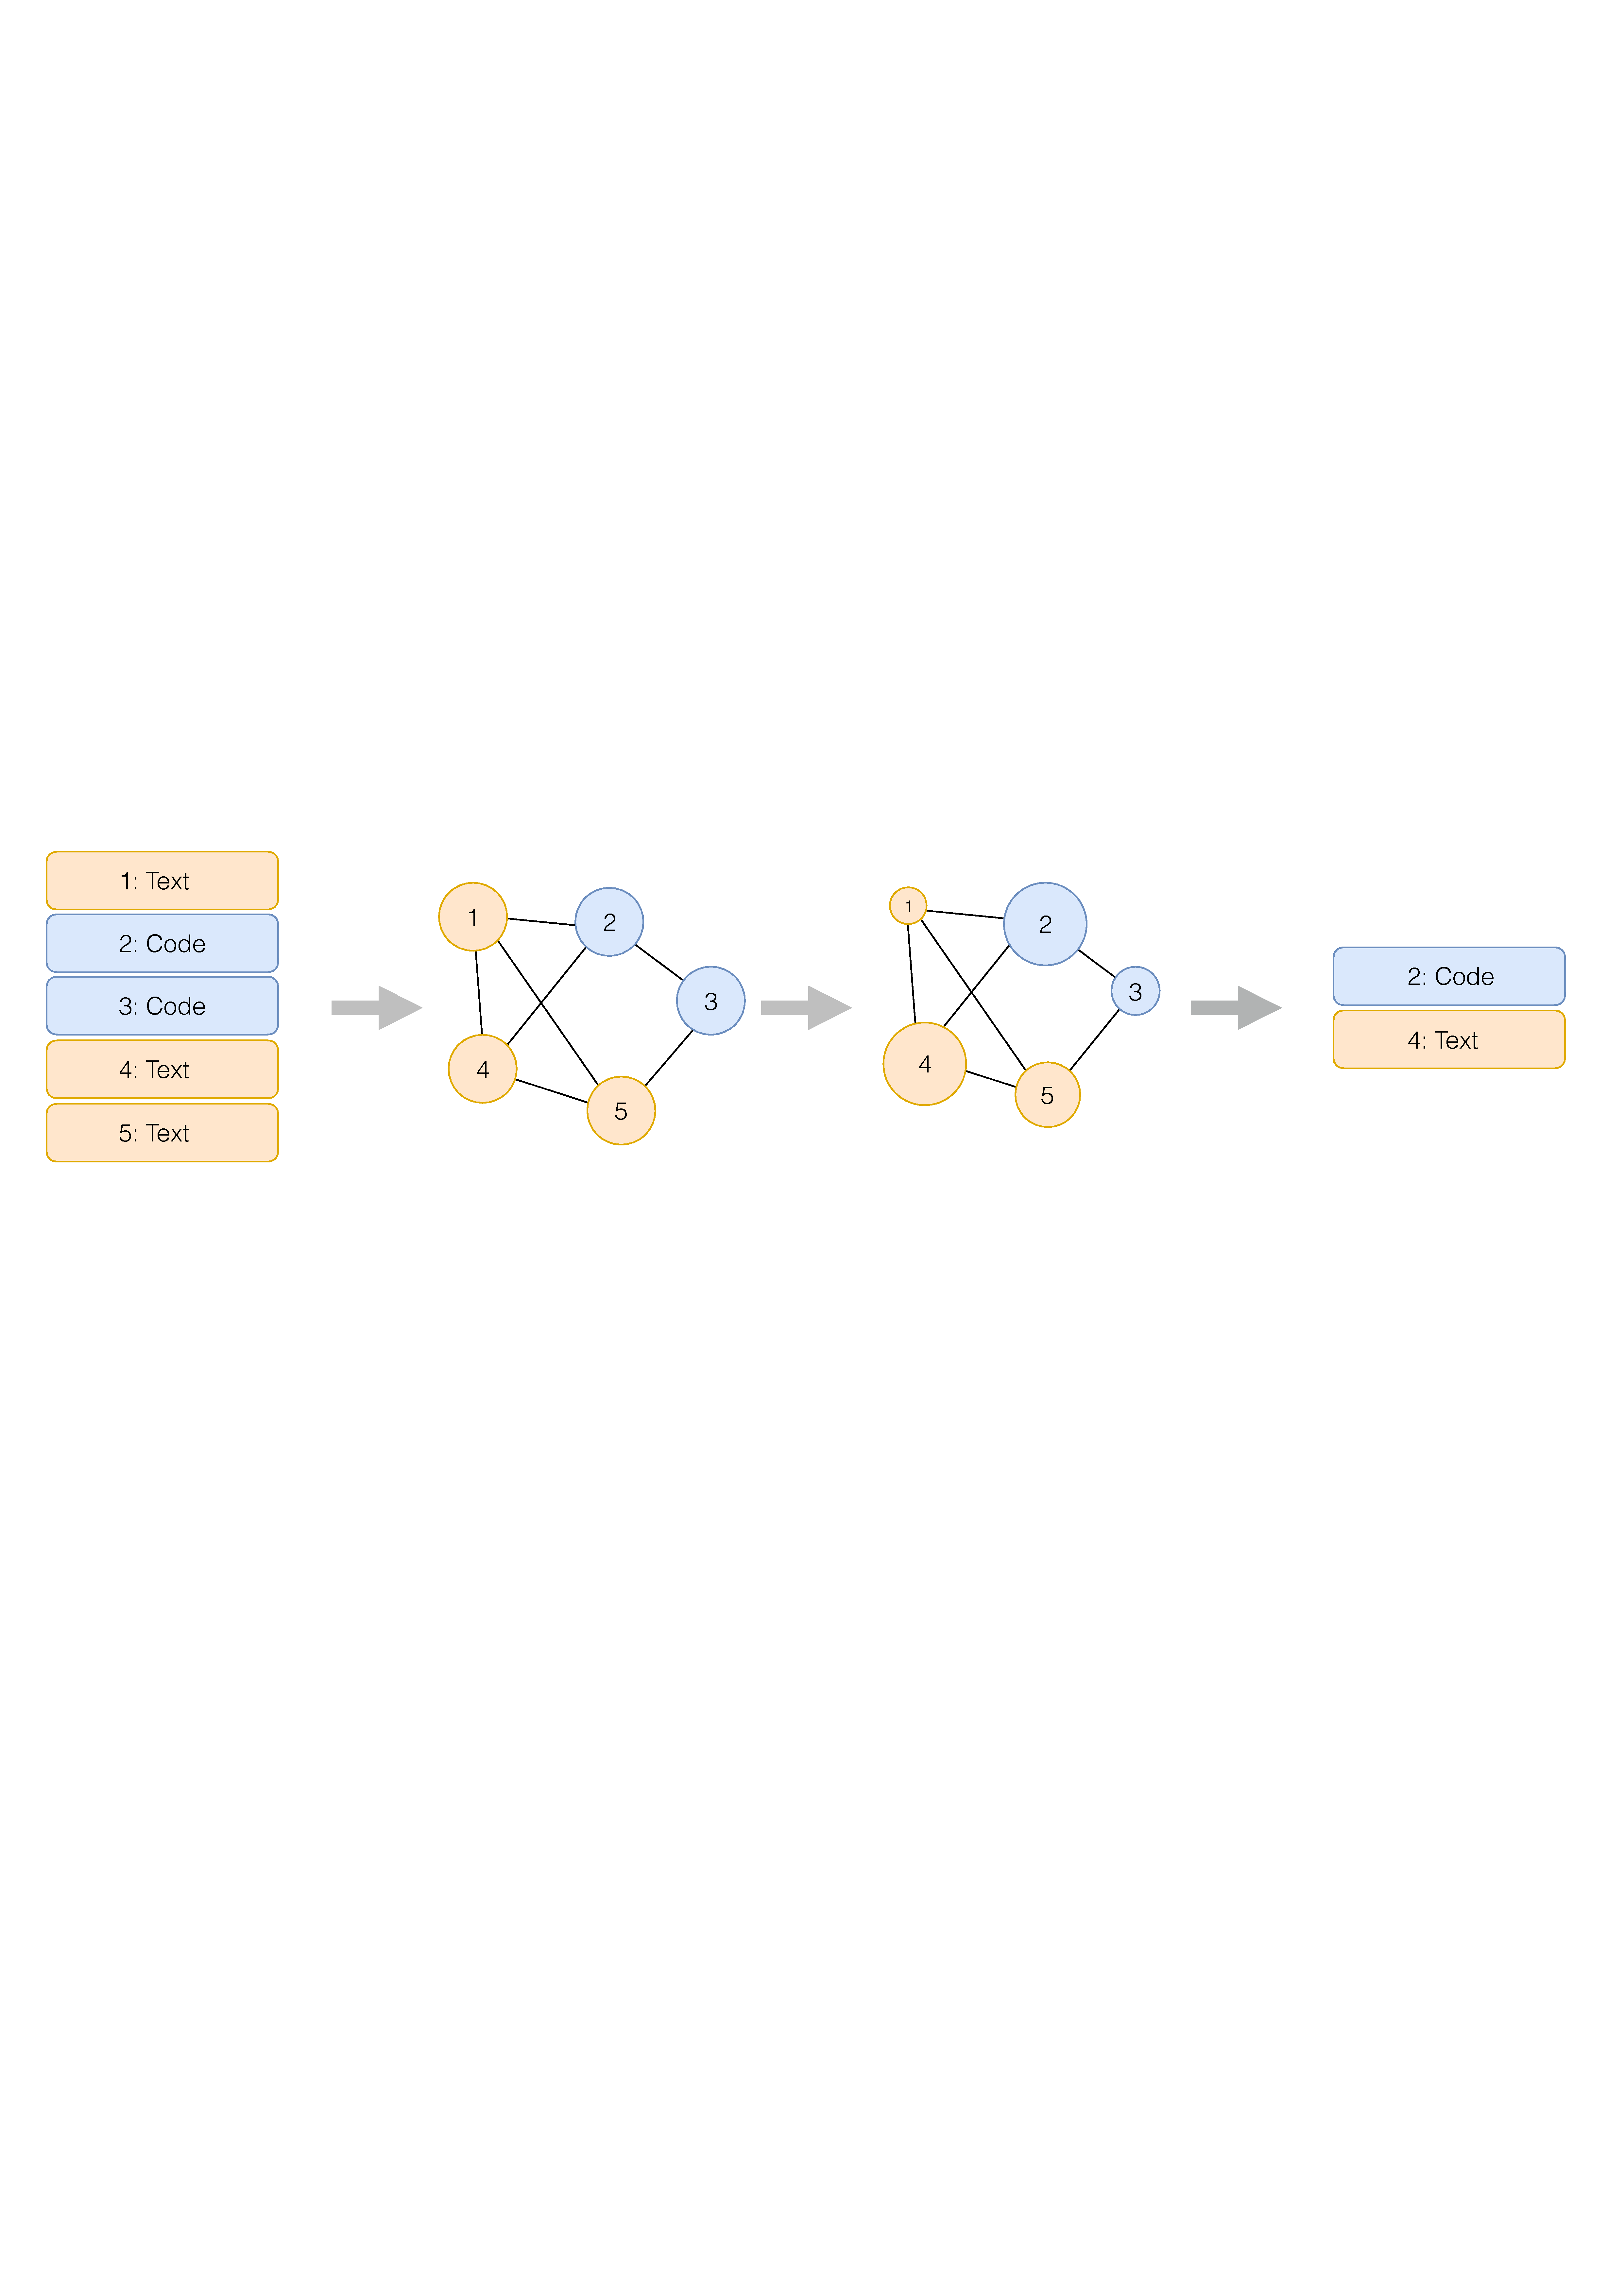
\includegraphics[scale=0.2]{Figures/graphs}
\caption{From website, to graph, to summary}
\label{fig:graph}
\end{figure} 

A major issue with this approach is the lack of context when creating the summary. In other words, the knowledge acquired by the user through the previously browsed pages is not considered while selecting the most relevant units.

In our implementation, we consider the history visited by a developer. We create a Context Graph ad-hoc for each developer which aggregates information units from different sources. When the developer visits a new page we extract the units from it, and add them to the graph. An example is shown in Figure \ref{fig:multipleDocumentGraph}.


\begin{figure}[H]
\centering
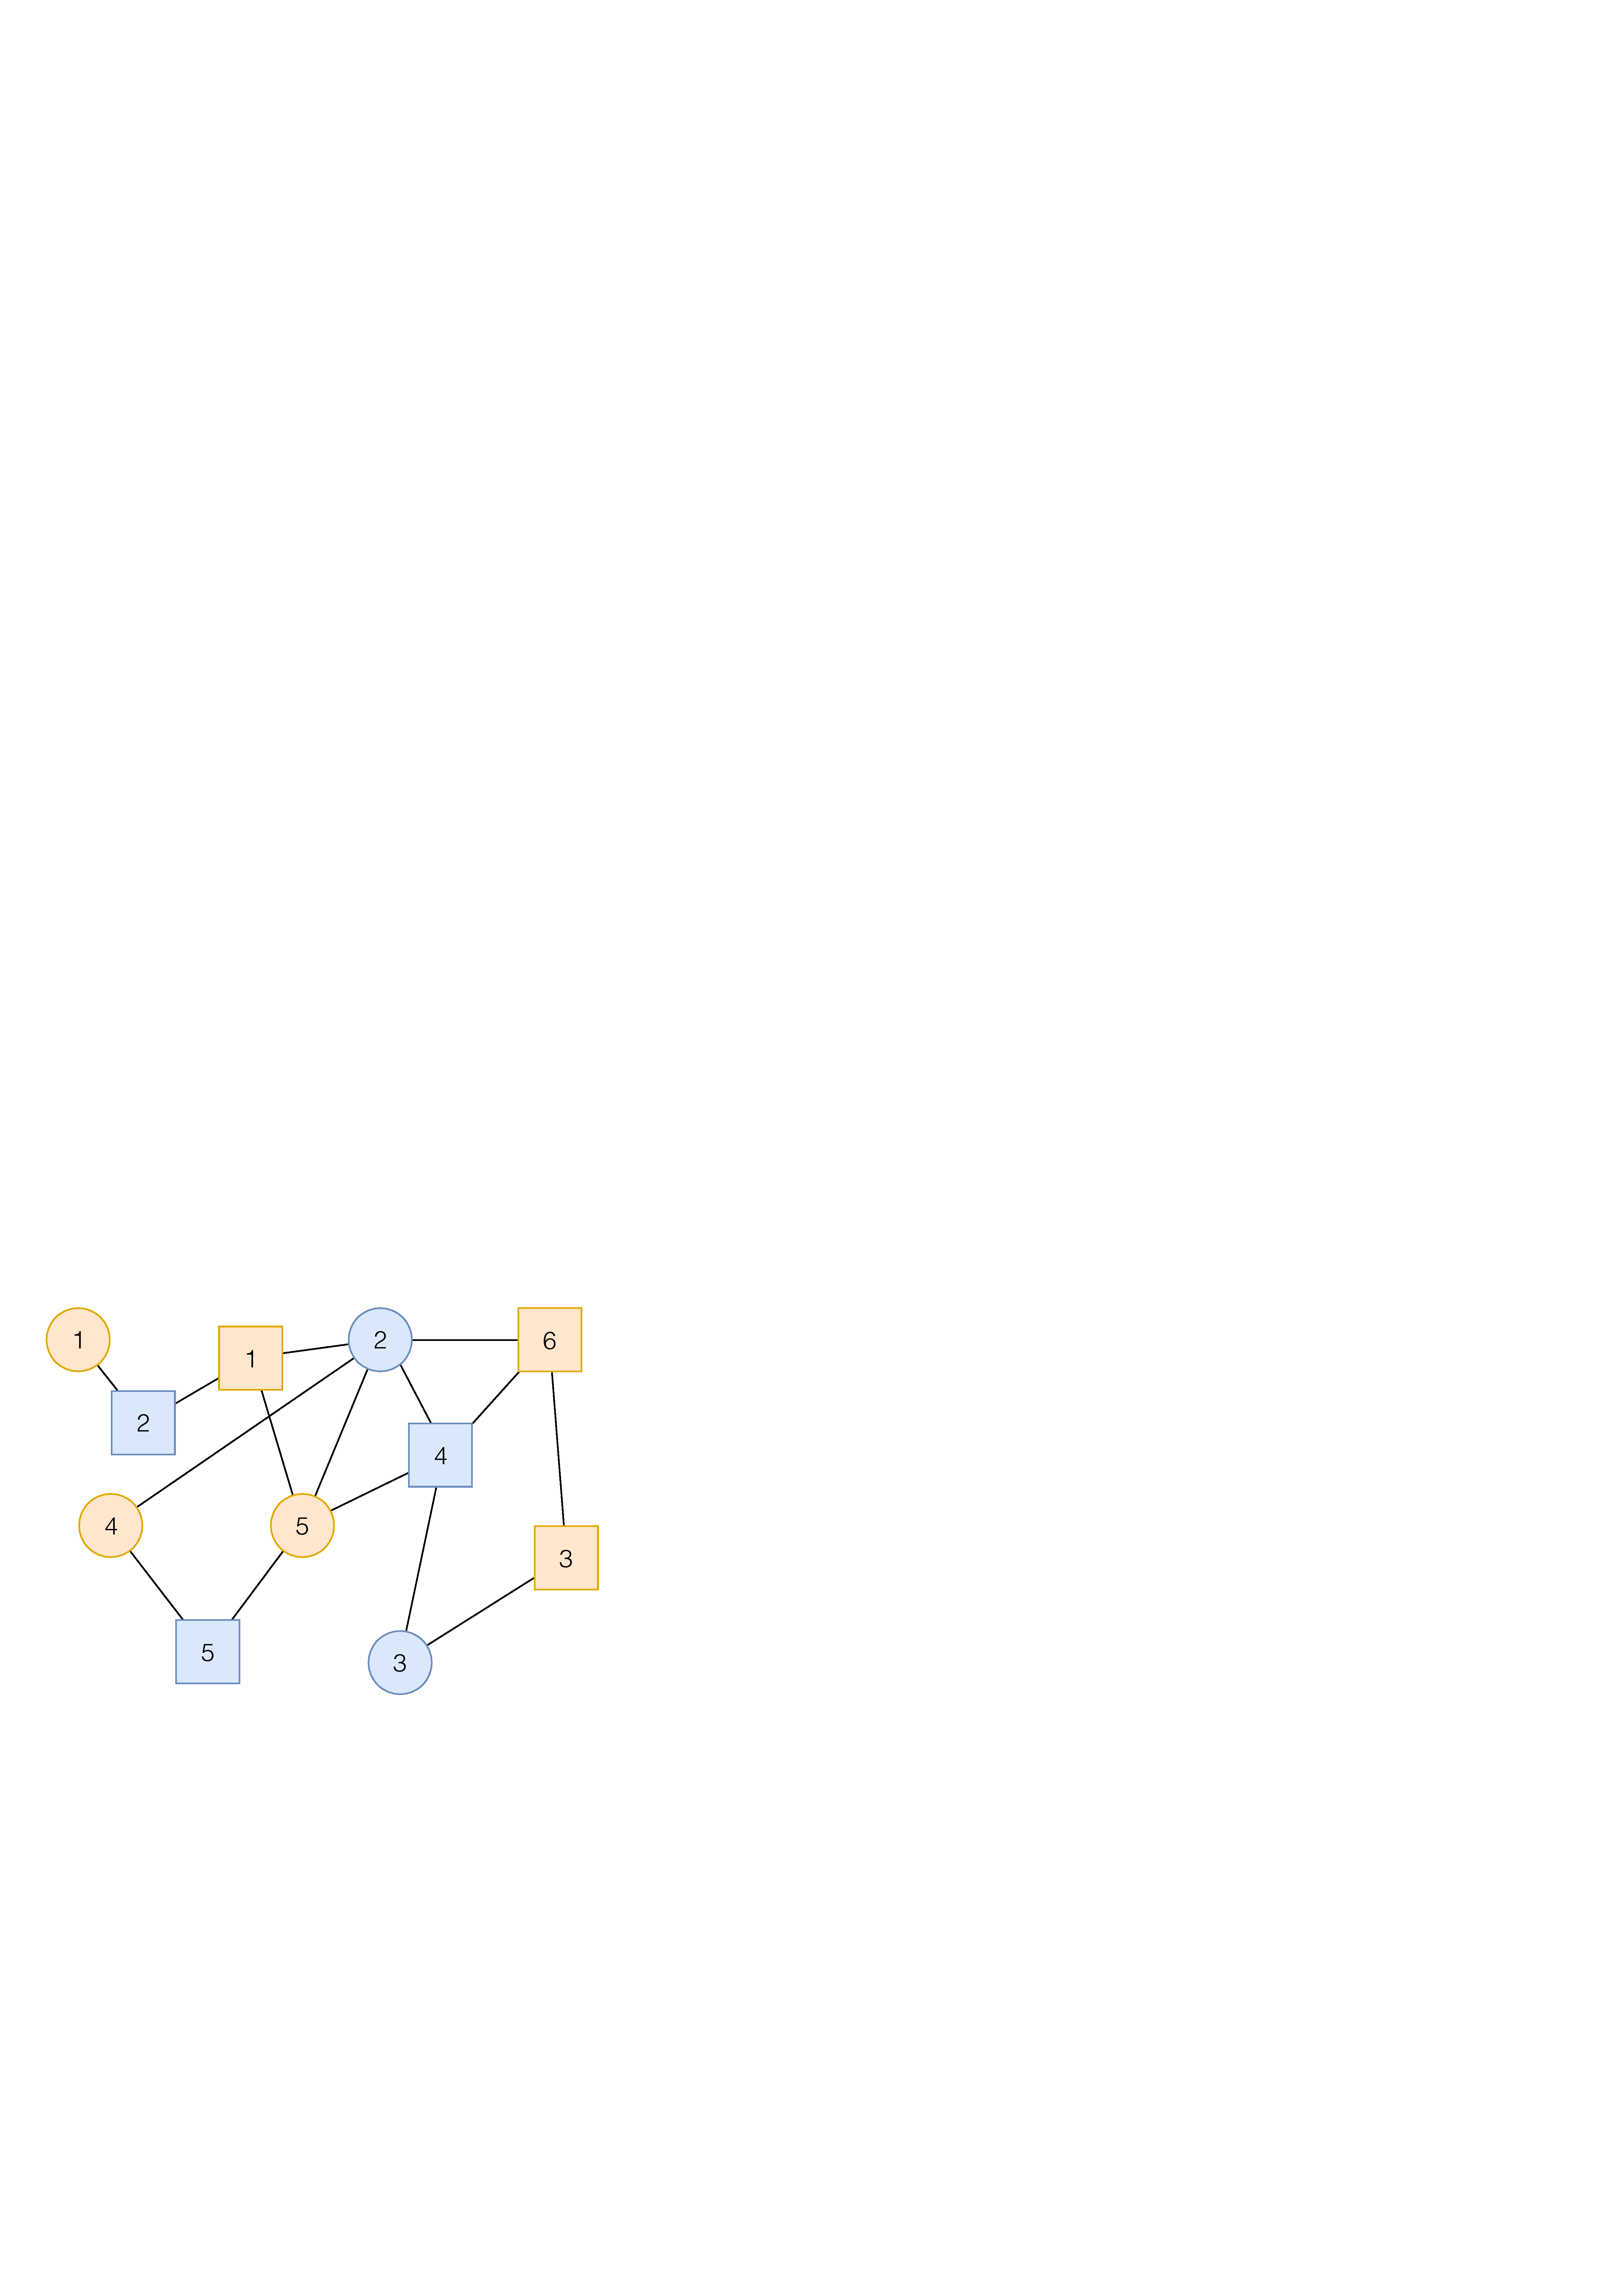
\includegraphics[scale=0.2]{Figures/mdGraphs}
\caption{Context graph}
\label{fig:multipleDocumentGraph}
\end{figure} 

In Figure \ref{fig:multipleDocumentGraph}, different sources are represented by different shapes (Squares represent document A, circles represent document B). When calculating the degree of centrality of a certain unit, the result is not based only on the content of the page currently being viewed, but it depends on all of the other units, which represent the history of pages visited. This means that anytime a new node is added to the context graph, the degree of a specific unit changes, as the context has changed. Therefore, a summary of a web page will change depending on the web pages visited.

\subsection{Architecture}\label{sec:architecture}
The project has two main components:
\begin{itemize}
\item \textbf{Chrome Web Extension}\\
Used to gather the information contained in a page by following the rules set up for a certain domain, as well as controlling the amount of information currently displayed
\item \textbf{Web Service}\\
Instead of relying on the end user's device to perform the calculations to determine the importance of each section, we developed a web service.
\end{itemize}

\begin{figure}[H]
\centering
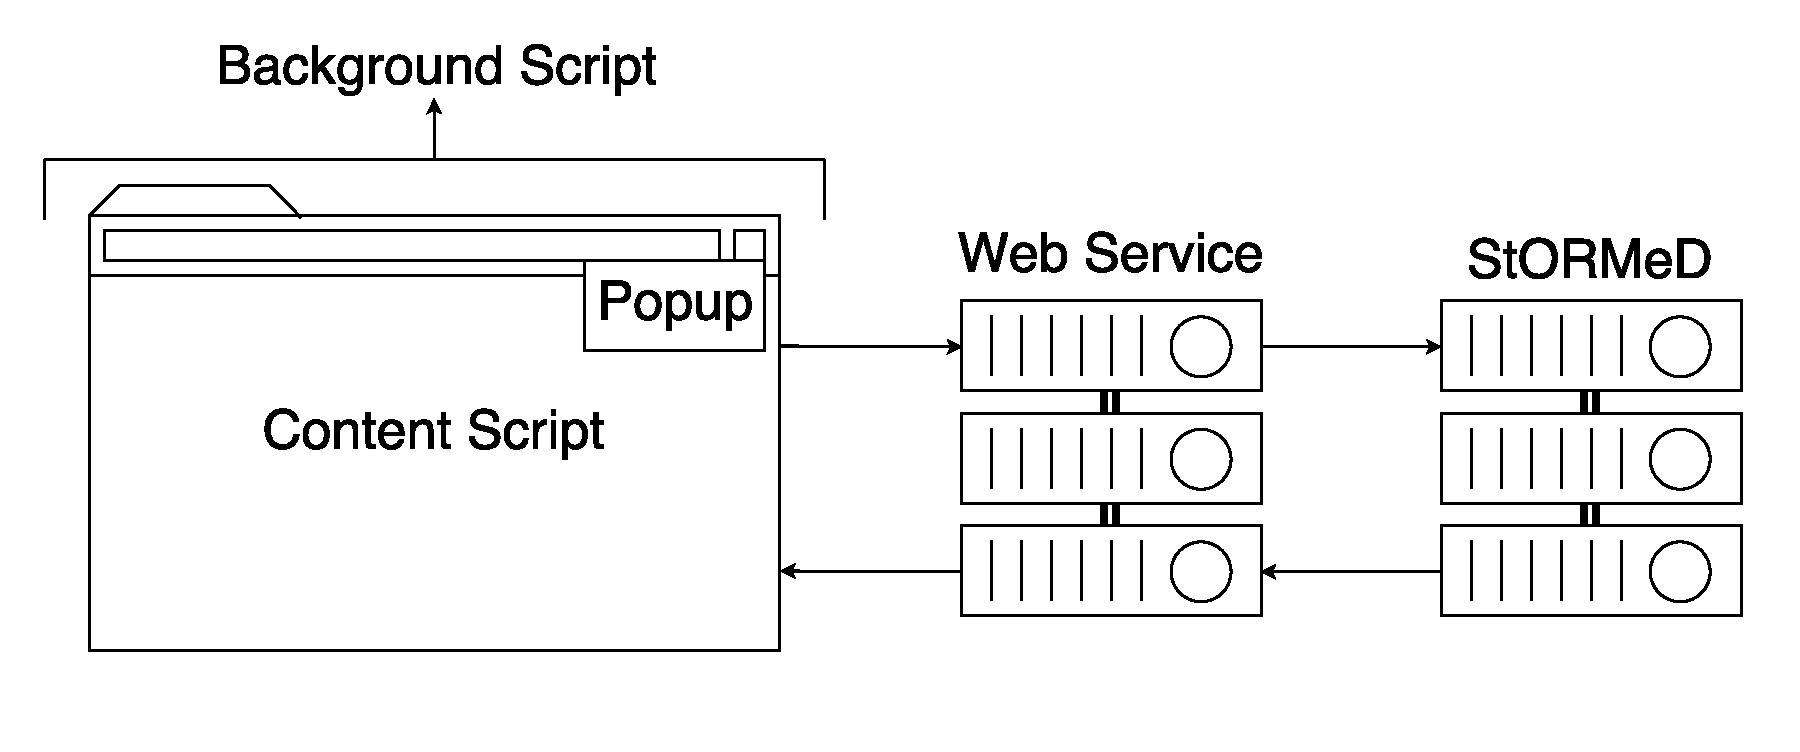
\includegraphics[scale=0.4]{Figures/ArchitectureNoLabel}
\caption{Architecture of \projectName}
\label{fig:architecture}
\end{figure} 
These two components interact with each other, in a typical client-server architecture, as shown in Figure \ref{fig:architecture}.


\begin{figure}[H]
\centering
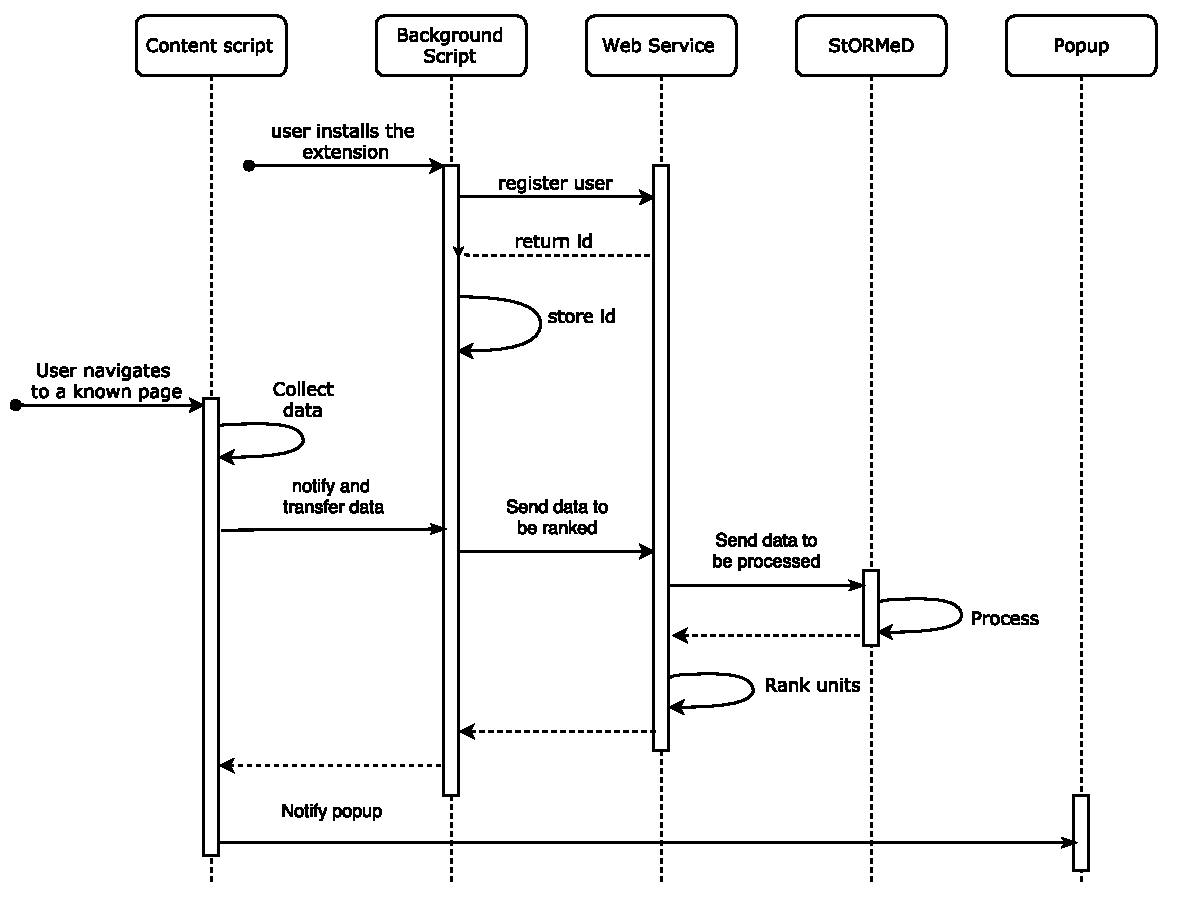
\includegraphics[scale=0.75]{Figures/SequenceDiagramAll}
\caption{Sequence diagram}
\label{fig:sequenceDiagram}
\end{figure}


Figure \ref{fig:sequenceDiagram} shows the sequence for both the registration procedure, as well as a normal request. For the registration, the procedure is as follows:
\begin{enumerate}
\item The user installs the extension, which triggers the registration request
\item The request is made to the service, which generates the user id and returns it to the client
\item The id is saved in in the local storage for the user
\end{enumerate}

\noindent Whereas for the ranking request, the procedure is as follows:
\begin{enumerate}
\item The user navigates to a known page, which triggers the data collection phase
\item The data is sent to the web service to be ranked
\item Units are processed, and a request is made to the StORMeD service
\item Once the data returns, the units are added to the user's graph, and the prominence is calculated
\item Ranked units are returned to the Chrome extension, which now allows the user to manipulate the information available on the page
\end{enumerate}

\subsection{Server side}
\subsubsection{Web Service}
The first component of this project consists in a web service, that takes the information units given by the extension, and returns the degree of centrality for each of the information units. This service was written in Scala, using the Play framework, and has the following routes:

\begin{itemize}
\item \texttt{GET /register}\\
Used to register the user to the service. This is needed to identify the user in all subsequent calls to the service. The response is a 32-character alphanumeric string, known as the user's id. Once the user registers, a graph is created unique to this id, allowing fadditional information units to be added, and therefore the ranking to be performed depending on the entire graph, not only the current units being analysed.
\item \texttt{POST /rank}\\
This path is used to rank the current units extracted from a document. By supplying the url of the webpage, the units, and the user id header, the service will return the units with a degree of centrality. 
\item \texttt{GET /all}\\
Returns the entire graph for a certain user, with all units associated with their degree of centrality.
\end{itemize}



To better understand how a request looks like, consider Listing \ref{lst:sampleRequest}. The user id that is created upon registration is attached to every request as a header as well as the URL of the page. 
\begin{listing}[H]
\centering	
\begin{jsoncode}
POST /rank
Content-Type: application/json
X-Libra-UserId: SsrktS2vrGPpHaAkYMsVDPo4qN6i38ei

{
  "units": [
    {
      "idx": "-656298628_0000000001",
      "parsedContent": "Creating an instance of a class:",
      "tags": [
        "plaintext"
      ]
    },
    {
      "idx": "-656298628_0000000002",
      "parsedContent": "MyObject myObject = new MyObject();",
      "tags": [
        "code"
      ]
    }
  ],
  "url": "http://www.mywebsite.io"
}
\end{jsoncode}
\caption{Sample request from Chrome extension to web service}
\label{lst:sampleRequest}
\end{listing}

As shown in the sequence diagram in Figure \ref{fig:sequenceDiagram}, an external call is made to the StORMeD service, an island parser which we use to construct an Heterogeneous Abstract Syntax Tree (H-AST)\cite{Ponz2017a} for all units. An H-AST is a structure that is used to represent both textual fragments as well as code fractions of an artifact. 

\begin{listing}[H]
\centering	
\begin{jsoncode}
{
  "units": [
    {
      "idx": "-656298628_0000000001",
      "degree": 0.5,
      "url": "http://www.mywebsite.io"
    },
    {
      "idx": "-656298628_0000000002",
      "degree": 0.5,
      "url": "http://www.mywebsite.io"
    }
  ]
}
\end{jsoncode}
\caption{Sample response}
\label{lst:sampleResponse}
\end{listing}

The service will then add the nodes to the graph, and calculates the degree by using a library called Signal/Collect\cite{Stutz:2010:SGA:1940281.1940330}, which allows high performance processing of large graphs. By describing the HoliRank algorithm using the provided syntax, the library handles the calculations returning the degree of centrality for a certain unit. The results are then returned to the user as seen in Listing \ref{lst:sampleResponse}.

This information is then used by the extension to associate the index with its degree, which is then used to decide which units have to be hidden and which have to be shown depending on the threshold chosen by the user. This is explained in details in the next section.

\subsubsection{StORMeD}
StORMeD\cite{Ponz2015a} is an island parser capable of building the Heterogeneous Abstract Syntax Tree (H-AST) for a piece of content. In out project, we use the service to analyze the code snippets which are parsed from the page. The web service makes a call to the StORMeD service, which returns the full H-AST that is fed into HoliRank.

\subsection{Client-side: Chrome extension}
\subsubsection{Parser}
The first step consists in collecting the information currently being displayed, which happens when the page has finished loading its content. As previously discussed in section \ref{sec:lackOfStructure}, one of the main challenges of this project was to handle the wide variety of structures among webpages, being as each page tends to use the same HTML constructs but widely differ in the implementation. This hurdle was solved by implementing a parser for each domain we target (i.e. Stack Overflow\footnote{\url{http://stackoverflow.com/}}, Spring Documentation\footnote{\url{http://docs.spring.io/spring/docs/current/spring-framework-reference/htmlsingle/}}, DZone\footnote{\url{http://dzone.com/}}, Android Documentation\footnote{\url{https://developer.android.com/guide/index.html}}).

Consider a Stack Overflow discussion, as in Figure \ref{fig:soConv}. A Stack Overflow discussion consists of a question, and a set of answers with their own set of comments. Therefore our parser needs to first obtain the question, more specifically the paragraphs and comments that make up such question, and then repeat the task for each of the possible answers. 

\begin{figure}[H]
\centering
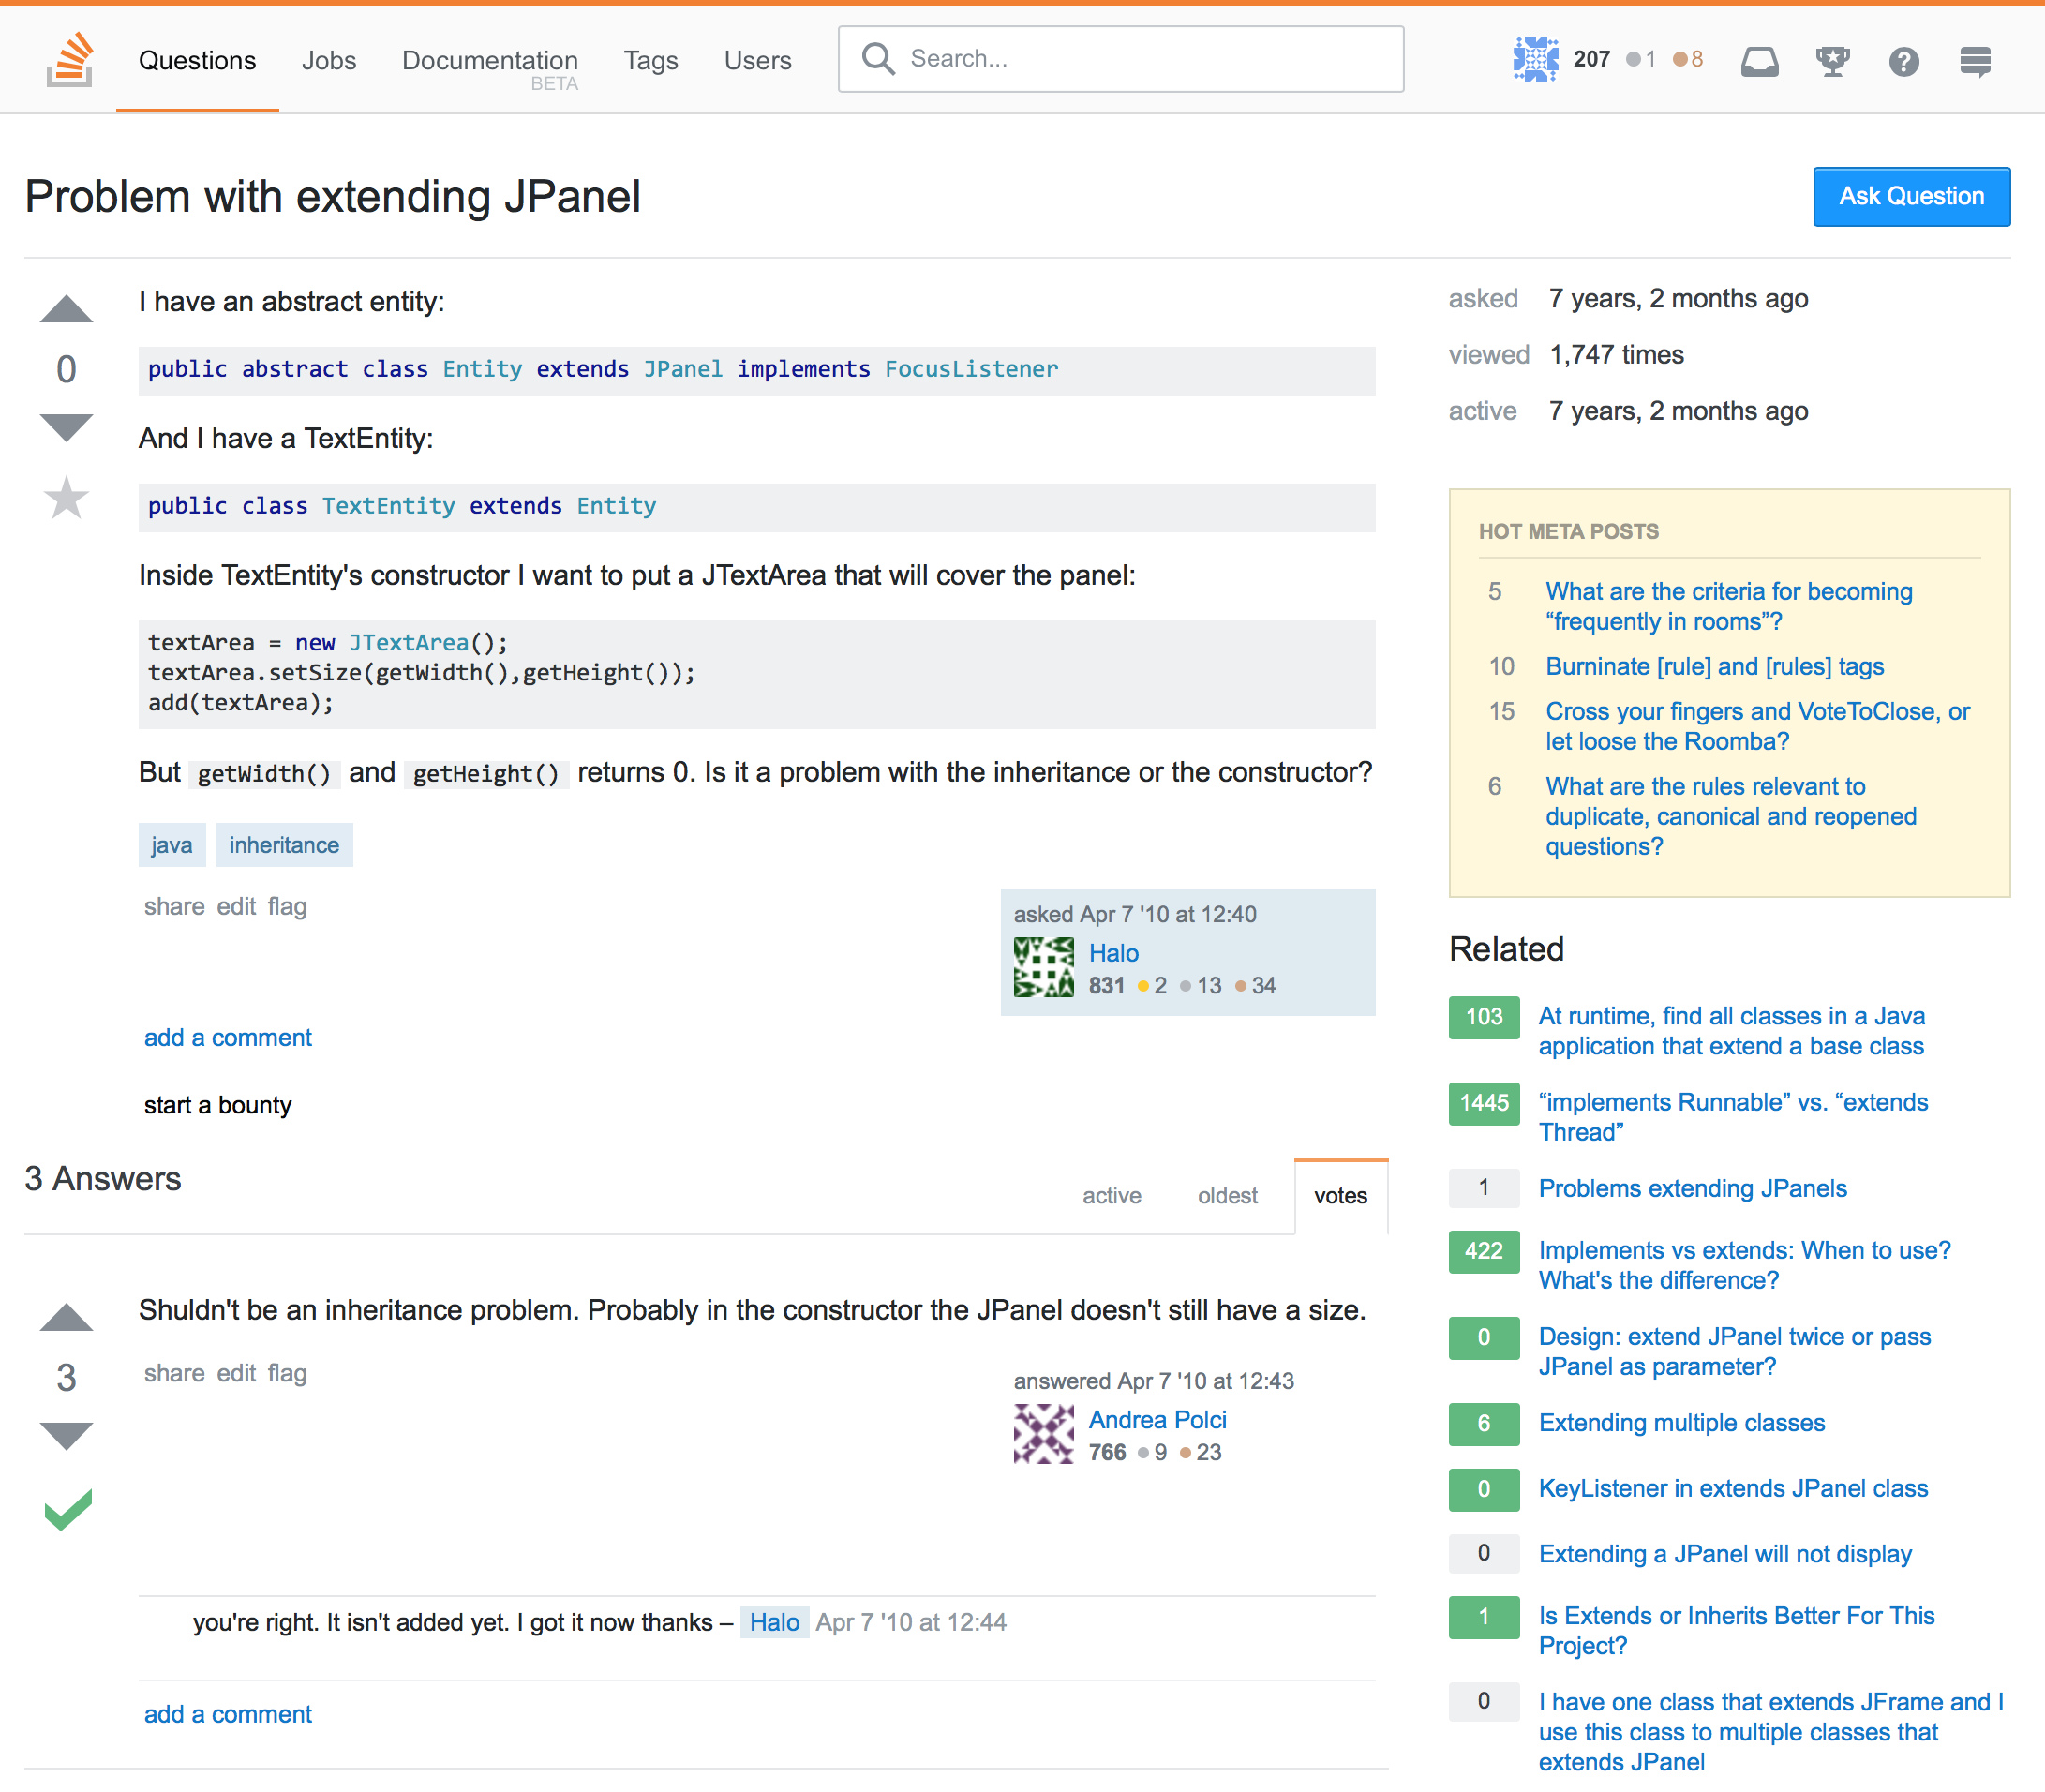
\includegraphics[scale=0.3]{Figures/SOConv}
\caption{A typical Stack Overflow discussion}
\label{fig:soConv}
\end{figure}

Since the structure of a Stack Overflow discussion differs from a tutorial from DZone\footnote{\url{http://dzone.com/}} , we needed to write a parser for each website we wish to parse. To facilitate this situation, we created an an abstract parser, along with a few standard models. We used TypeScript\footnote{\url{https://www.typescriptlang.org}}, a language developed by Microsoft which is a typed superset of JavaScript that compiles to plain JavaScript. This ensured that compatibility would not be an issue, while providing multiple useful features. We started by defining the models that would be needed to parse a page, in a very general way. A document diagram can be found in Figure \ref{fig:abstractParserClassDiagram}.

\begin{figure}[H]
\centering
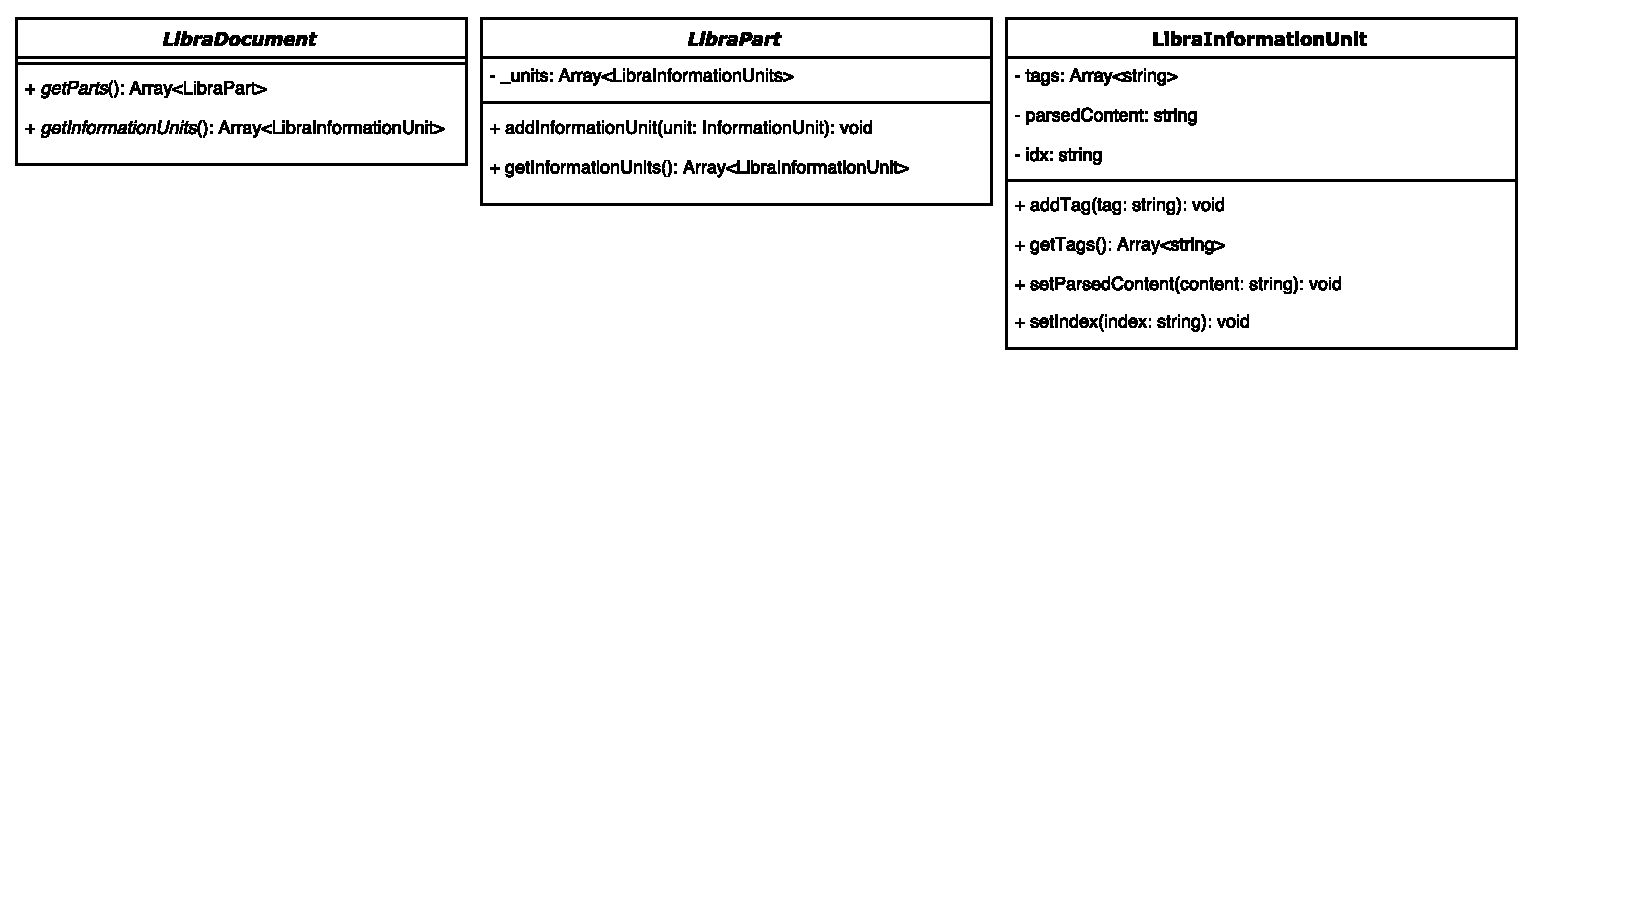
\includegraphics[scale=0.5]{Figures/ClassUML}
\caption{Abstract parser class diagram}
\label{fig:abstractParserClassDiagram}
\end{figure}

The ``root'' model is called \ts{LibraDocument} which provides the main methods called by the Chrome extension, namely \ts{parse()} and \ts{getInformationUnits()}. 

In our implementation of the information unit, called \ts{LibraInformationUnit}, we also store a few other useful parts such as the index of the unit and the tags attached to the DOM. 

The last component is \ts{LibraPart}, which separates the multiple parts of a document.


%As an example, consider the Stack Overflow discussion shown in Figure \ref{fig:soConv}. We could divide the question and the answers in two separate parts, which in turn  contain other parts (i.e. the possible comments to a question or answer). 

\begin{figure}[H]
\centering
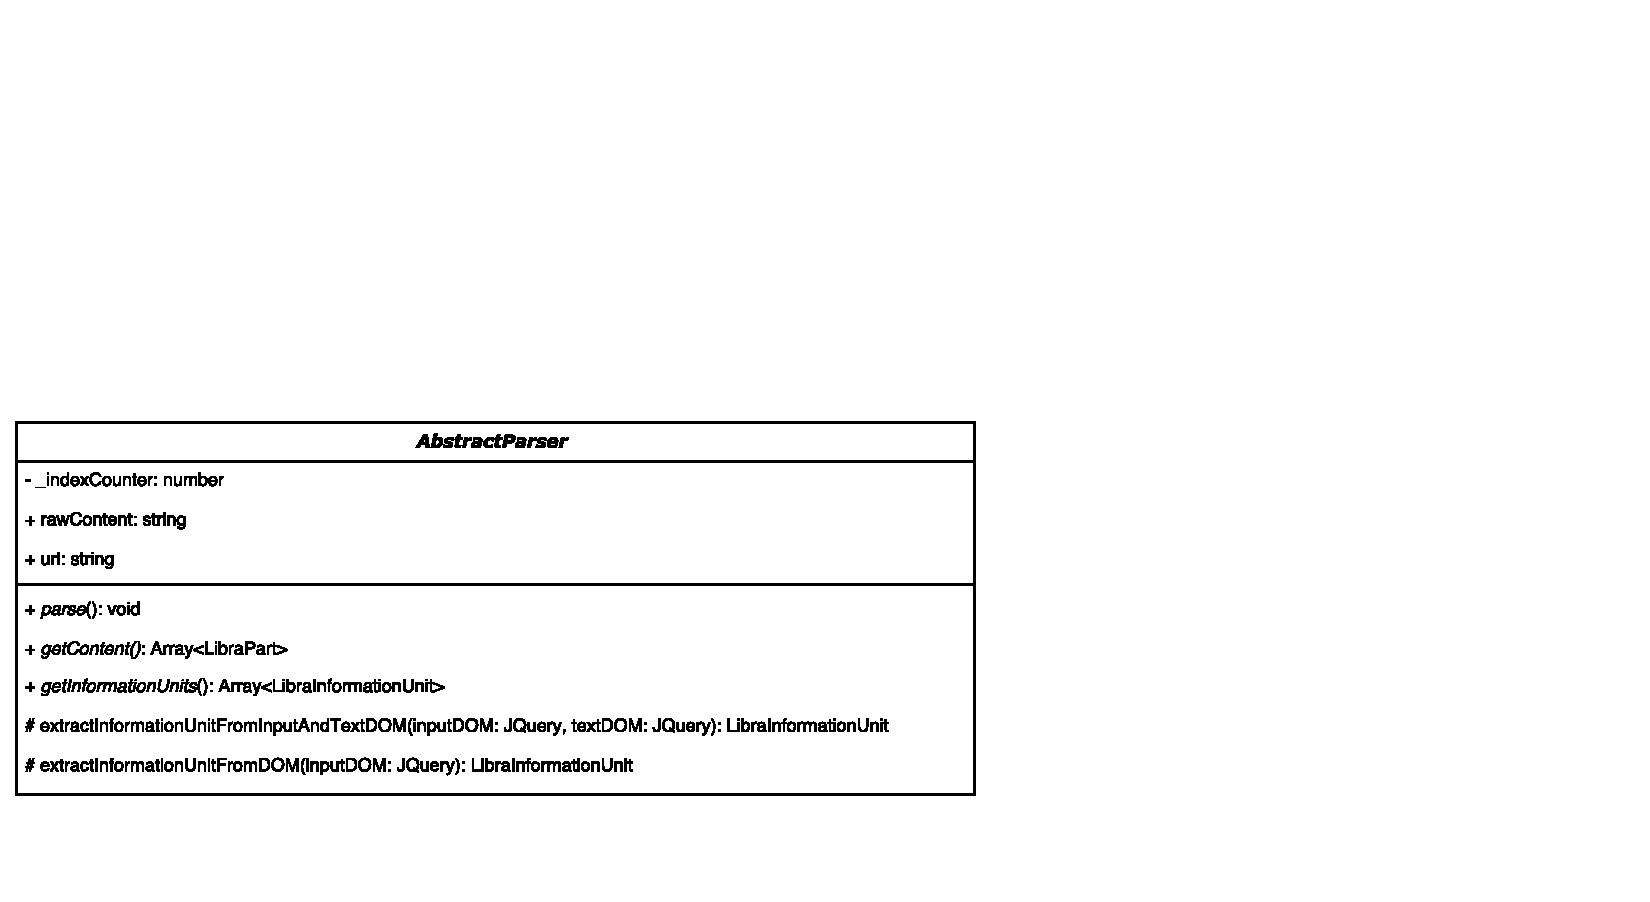
\includegraphics[scale=0.5]{Figures/AbstractParserUML}
\caption{Abstract parser}
\label{fig:abstractParserDiagram}
\end{figure}

These models are then used in the abstract parser (see diagram in Figure \ref{fig:abstractParserDiagram}). This way the developer writing a new parser has to simply extend the different methods and models. 

A remark has to be made about the \ts{extractInformationUnitFromInputAndTextDOM} and \\\ts{extractInformationUnitFromDOM} methods. These two methods were created to keep the data extracted consistent among multiple parser implementations. The consistency is achieved by requiring the DOM element that contains the artifact to be extracted, and returning a ready to use \ts{LibraInformationUnit}. What is hidden behind this implementation is a tagging procedure that allows the Chrome extension to connect the data returned by the service with the content being displayed. To provide a unique identifier for each of the elements on the page, we used a combination of the page's URL with a global counter. The structure of this index is as follows:
\[
\text{\texttt{Hash of url + "\_" + 10 digit padded counter}}
\]
When extracting the content of the DOM, the two previously mentioned methods inject the index into the DOM of the page as seen in Listing \ref{lst:sampleInjection}.
\begin{listing}[H]
\centering
\begin{htmlcode}
<pre class="lang-java prettyprint prettyprinted" libra_idx="-656298628_0000000001">
    ...
</pre>
\end{htmlcode}
\caption{Index injection example}
\label{lst:sampleInjection}
\end{listing}

Then, when the service has returned the degree of centrality associated with a certain index, we can perform a simple search inside of the page and link the data to the related DOM. 

Although hashing may introduce cases where the produced hash is not unique, the probability of such an event occurring is small enough to be ignored.

%By creating \ts{parse()} and \ts{getInformationUnits()} in \ts{LibraDocument} as abstract, each parser can implement their own, while allowing the extension to call the same methods, regardless of the page being viewed (and hence parser being used), while effectively providing a common interface to the parser. 

The execution of the parser is performed once the loading of the page is completed, which itself fires the request to the web service, discussed in the next section.


\subsubsection{Chrome Extension components}
A Chrome extension was created to parse the contents of a page, send it to the service, and then manipulate it. The  typical structure of a Chrome extension is divided into three components:
\begin{itemize}
\item \textbf{Background script}\\
The background script runs in the background for the whole browser, and is persistent. The session is not unique to the tab, and therefore no data exclusive to a certain tab should be stored in here.
\item \textbf{Popup}\\
The interface of the extension. It allows the developer to create a user interface, which can be shown every time the icon of the extension is clicked. It is important to notice that the user interface is created every time the icon for the extension is clicked, and completely destroyed once the user is not interacting with it anymore. 
\item \textbf{Content script}\\
The content script has access to the data currently being displayed. It is able to interact with the DOM, and its session is unique to each tab open. 
\end{itemize}
Each of these components has a very distinct and precise task. In order to make our extension work, all three components were implemented. 

Since each component of the extension has a different set of restrictions, the jobs have to be delegated to the component designed to perform it. Chrome uses message passing, a method where the different components can subscribe to receive certain types of messages, and have the ability to broadcast messages themselves to the other components. In our case, the three components were used in the following way:
\begin{itemize}
\item \textbf{Content Script}\\
The content script is responsible of loading the available parsers, as well as using the correct one for the current page. Once this is completed, the data is handed over to the background script.
\item \textbf{Background script}\\
The background script is responsible of connecting the content script with the popup, as well as making the HTTP requests to the service. 
\item \textbf{Popup}\\
The popup is shown containing a range slider, which allows the user to interact with the information being currently displayed on the page, and to manipulate it. 
\end{itemize}

As previously explained, message passing is the way components communicate with each other. This feature was used, for example, when the user had just registered to the service. Each component has its own local storage, but the user id had to be used by multiple components which created an issue regarding where to store it. In the end, message passing was used and a common local storage was chosen, this being the background script's storage as this component was always listening and active.






As we have seen in the previous section, the service returns the payload containing the different degrees of each unit. It is the task of the extension as a whole to process this information, and make it usable to the user. This is achieved by sorting the payload data, and adding in each of the units currently on the page a sort order index as seen in Listing \ref{lst:sampleSortOrderInjection}.
\begin{listing}[H]
\centering
\begin{htmlcode}
<pre class="lang-java prettyprint prettyprinted" libra_idx="-656298628_0000000001" sortorder="15">
	...
</pre>	
\end{htmlcode}
\caption{Sort order tag injection}
\label{lst:sampleSortOrderInjection}
\end{listing}
\noindent In the next section, we describe the resulting application, with an in depth explanation of the functionality.
